\documentclass[abstract=on,10pt,a4paper,bibliography=totocnumbered]{article}
\usepackage[paper=a4paper,left=35mm,right=35mm,top=25mm,bottom=30mm]{geometry}
\usepackage[doublespacing]{setspace}
\usepackage[english]{babel}
\usepackage[utf8]{inputenc}
\usepackage[round]{natbib}
\usepackage{amsmath}
\usepackage{colortbl}
\usepackage{amsfonts}
\usepackage{amssymb}
\usepackage{gensymb}
\usepackage{graphicx}
\usepackage{tikz}
\usepackage{enumerate}
\usepackage{enumitem}
\usepackage{subcaption}
\usepackage{booktabs}
\usepackage[hidelinks]{hyperref}
\usepackage[nameinlink]{cleveref}
% \usepackage{lineno}
\usepackage{multirow}
\usepackage{arydshln}
\usepackage[flushleft]{threeparttable}
\usepackage[nomarkers, nolists]{endfloat}
\usepackage[colorinlistoftodos]{todonotes}
\usepackage{scalerel}
\usepackage{tikz}
\usetikzlibrary{svg.path}

%------------------------------------------------------------------------------
%	Some Styling
%------------------------------------------------------------------------------
% Creating some TikZ styles
\tikzset{
  nonterminal/.style = {rectangle
    , minimum size = 6mm
    , very thick
    , draw = black!
  }
}

% Changing the style of captions in figures etc.
\captionsetup{labelfont=bf, format=plain, font=small}

% Change how equations are referenced
\renewcommand{\theequation}{Equation \arabic{equation}}%

% To be able to put an ORCID
\definecolor{orcidlogocol}{HTML}{A6CE39}
\tikzset{
  orcidlogo/.pic={
    \fill[orcidlogocol] svg{M256,128c0,70.7-57.3,128-128,128C57.3,256,0,198.7,0,128C0,57.3,57.3,0,128,0C198.7,0,256,57.3,256,128z};
    \fill[white] svg{M86.3,186.2H70.9V79.1h15.4v48.4V186.2z}
                 svg{M108.9,79.1h41.6c39.6,0,57,28.3,57,53.6c0,27.5-21.5,53.6-56.8,53.6h-41.8V79.1z M124.3,172.4h24.5c34.9,0,42.9-26.5,42.9-39.7c0-21.5-13.7-39.7-43.7-39.7h-23.7V172.4z}
                 svg{M88.7,56.8c0,5.5-4.5,10.1-10.1,10.1c-5.6,0-10.1-4.6-10.1-10.1c0-5.6,4.5-10.1,10.1-10.1C84.2,46.7,88.7,51.3,88.7,56.8z};
  }
}
\newcommand\orcid[1]{\href{https://orcid.org/#1}{\mbox{\scalerel*{

\begin{tikzpicture}[yscale=-1,transform shape]
  \pic{orcidlogo};
\end{tikzpicture}
}{|}}}}

%------------------------------------------------------------------------------
%	Titlepage: Header
%------------------------------------------------------------------------------
\title{Flooding of the Okavango Delta influences Connectivity for Dispersing
African Wild Dogs}

% List of Authors
\author{
  David D. Hofmann\textsuperscript{1,2,\S} \orcid{0000-0003-3477-4365} \and
  Gabriele Cozzi\textsuperscript{1,2} \orcid{0000-0002-1744-1940} \and
  John W. McNutt\textsuperscript{2} \and
  Arpat Ozgul\textsuperscript{1} \orcid{0000-0001-7477-2642} \and
  Dominik M. Behr\textsuperscript{1,2} \orcid{0000-0001-7378-8538}
}

% Reduce spacing between authors
\makeatletter
\def\and{%
  \end{tabular}%
  \hskip -0.5em \@plus.17fil\relax
  \begin{tabular}[t]{c}}
\makeatother

% Current Date
% \date{\today}

% And here the masterpiece begins
\begin{document}

% Change page numbering
\pagenumbering{gobble}

% Required to be able to cite
\bibliographystyle{apalike}

% Create Titlepage
\maketitle

%------------------------------------------------------------------------------
%	Titlepage: Additional Info
%------------------------------------------------------------------------------
\begin{flushleft}

\vspace{0.5cm}

\textsuperscript{1} Department of Evolutionary Biology and Environmental
Studies, University of Zurich, Winterthurerstarsse 190, 8057 Zurich,
Switzerland.

\textsuperscript{2} Botswana Predator Conservation Program, Private Bag 13,
Maun, Botswana.

\textsuperscript{\S} Corresponding author (david.hofmann2@uzh.ch)

\vspace{4cm}

\textbf{Running Title:} None

\vspace{0.5cm}

\textbf{Keywords:} Seasonal Flooding of the Okavango Delta and its Consequences
for African Wild Dog Connectivity

\end{flushleft}

%------------------------------------------------------------------------------
%	Abstract
%------------------------------------------------------------------------------
\newpage
\begin{abstract}
Climate change is expected to profoundly impact vital rates of wild living
animal populations. While the impact of climate change on the demographics of
local subpopulations has been studied repeatedly, little is known about the
consequences of environmental change on dispersal and connectivity between such
subpopulations.

Here, we capitalize on natural, flood-pulse driven environmental change across
the Okavando Deltas in northern Botswana to investigate the impact of changing
environmental conditions on the dispersal ability of the endangered African wild
dog. For this, we utilize a previously parametrized dispersal model and apply it
to simulate dispersal under two extreme environmental scenarios; one assuming
minimal flood extent, one assuming maximum flood extent.

In genral, our results suggest only a marginal impact of the flood extent on
dispersal prospects. Even during maximum flood, dispersal between neighboring
patches remained high. Between a few selected patches, however, dispersal was
substantially restricted during times of high flood. That is the Okavango delta
posed a substantial dispersal barrier that reduced connectivity between patches
during maximum flood, but revealed vital dispersal corridors that facilitated
dispersal into neighboring areas during minimum flood. Besides a better
understanding of the conservation needs for the African wild dog, our study also
presents a first step towards incorporating environmental change due to
seasonality or climate change. It also emphasizes the usefulness of
individual-based dispersal simulations as a conservation tool to study impacts
of environmental change in a spatially realistic way.

\end{abstract}

%------------------------------------------------------------------------------
%	Main Text
%------------------------------------------------------------------------------
\newpage

\onehalfspacing
\tableofcontents
\doublespacing

% Change page numbering
\newpage
\pagenumbering{arabic}

% Create linenumbers
% \linenumbers

\section{Introduction}
\subsection{Climate Change}

Despite the importance of climate change in determining species viability,
predicting the way and extent to which it will affect species remains
challenging. One exciting avenue to gain insights into the implications of
environmental change is to utilize seasonal variation in the environment.

Cite IPCC, Planetary boundaries, Tucker (step length). Phenological shifts. Cite
Robynne, Arpat, Megan, Dominik, Rabaiotti etc.

\subsection{Vital Rates}
Several studies investigating the impacts of climate change on life-history
traits have revealed that population persistence may critically depends on
climate conditions \citep{Paniw.2019}. While many studies examine climate
impacts on survival and reproductive rates, the influence of global change or
climatic extreme events on dispersal prospects has received little attention.

Ecosystems that undergoe seasonal environmental variation, in particular arid
regions that experience extreme climatic conditions, are among the most
vulnerable to climate change.

\subsection{Dispersal}
\subsection{Connectivity}
Dispersal is an important, if not the important, driver of landscape
connectivity and therefore of major interest to conservation authorities.

\subsection{Okavango Delta and African Wild Dogs}
The Okavango delta in Southern Africa poses a unique opportunity to study the
impacts of environmetal change on species dispersal ability and connectivity in
large scale natural experiment setup. According to projections by the IPCC,
Botswana and its surroundings are among the most vulnerable to climate change.


\section{Methods}
We conducted all analyses using the programming language R.

\subsection{Study Area}
The study area for this analysis was focused on the Okavango delta and its
surroundings in Southern Africa, comprising parts of Angola, Namibia, Botswana,
Zimbabwe, and Zambia (\Cref{StudyArea}). To accommodate for the long distance
dispersal events commonly observed in African wild dogs (e.g.
\citep{DaviesMostert.2012, Masenga.2016, Cozzi.2020}), we considered a large
rectangular extent stretching from 20\degree 30' E to 26\degree E. totaling to
an area of 300'000 km\textsuperscript{2}. The dominant geographical feature in
this region is the Okavango delta (OD), the world's largest inland delta and the
main driver of seasonal environmental change in the region. The flood-pulsing
rhythm of the OD is mainly dictated by precipitation in the Angolian highlands,
where rainfalls are channeled into the OD through the Okavango River. Although
precipitation in Angola peaks in ..., water only slowly descends through the
Okavango river and its tributaries, reaching the distal ends (i.e. the faults)
of the delta in July or August. At minimum extent, the flood covers an area of
3'600 km\textsuperscript{2}, whereas during maximum flood it covers more than
9'000 km\textsuperscript{2}. Vegetation in the study area is dominated by dense
mopane forest, mixed acacia woodland, and plain grassland. Human influence in
the study area is low and mainly concentrated around small villages at the
western periphery of the delta and to the city of Maun at the southern tip of
the delta. Large portions of land are dedicated national parks, game reserves or
forest reserves. The study area is also part of the world's largest
transboundary conservation initiative, the Kavango-Zambezi Transfrontier
Conservation Area.

\begin{figure}
  \begin{center}
  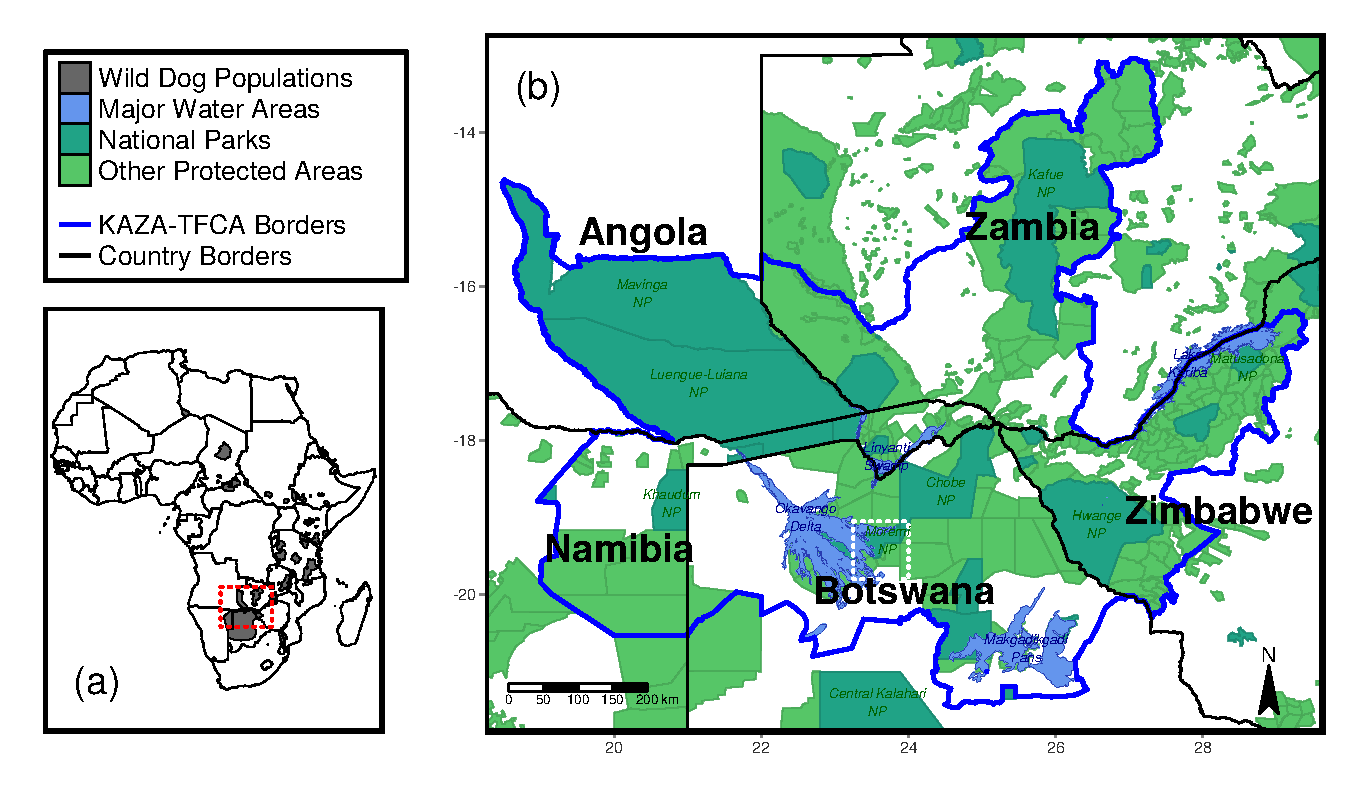
\includegraphics[width = \textwidth]{99_StudyArea.png}
  \caption{Study area across which we simulated dispersal events. Virtual
  dispersers were released at random locations within the orange source areas.}
  \label{StudyArea}
  \end{center}
\end{figure}

\subsection{Spatial Habitat Layers}
We represented the physical landscape through which dispersers could move by a
set of spatially referenced habitat layers each resolve at 250m x 250m. The set
of layers included water-cover, distance-to-water, tree-cover,
shrub/grassland-cover, and a human influence layer depicting anthropogenic
influences through villages, roads, and agriculture. A detailed description of
the different layers is provided in \Cref{Hofmann.2021}. Importantly, the
water-cover and the derived distance-to water layers were generated using MODIS
Terra satellite imagery, which enabled us to generate weekly updated layers that
provided detailed information about the flood-extent at any given point in time.
We had a total of 8xx remote sensed floodmaps at our disposal and used them to
generate two extreme scenarios; a minimal and maximum flood scenario. To create
the minimum flood scenario, we tallied the 50 floodmaps with smallest flood
extent into an average image. Finally, we created a binary map... Similarly, we
created an average image for high flood using the 50 most flooded maps. The
resulting maps are depicted in \Cref{FloodExtent}. For completeness we also
generated an  ``average'' floodmap by averaging across all 800 floodmaps
available to us. The results based upond this layer are presented in the
Appendix.

\begin{figure}
  \begin{center}
  \includegraphics[width = \textwidth]{99_FloodExtent.png}
  \caption{}
  \label{FloodExtent}
  \end{center}
\end{figure}

\subsection{Dispersal Model}
Our dispersal model was based on a previously parametrized and validated
\textit{integrated step-selection function (iSSF)} applied to the dispersal data
of 16 dispersing African wild dogs inhabiting the surroundings of the Moremi
National Park in the Okavango delta \citep{Hofmann.2021}. The iSSF model
consists of two complementary ``kernels'' plus their interactions. The first
kernel is a movement kernel and describes general movement behavior of
dispersing AWDs, irrespective of habitat conditions. The second kernel is a
habitat kernel and describes preferences of AWDs with regards to environmental
conditions. Finally, the model also includes interactions among the two kernels
and therefore allows to render how movement behavior changes depending on
habitat conditions.

\subsection{Source Areas}
We simulated dispersing AWDs originating from nine distinct source patches
located in the vicinity of the Okavango delta. The source areas were generated
as follows. First, we overlayed the OD with an oval that was bound by
geographical landmarks; in the north, the oval was bound by the Inflow of the
Okavango river into the ``pan-handle'' of the OD, north-east the oval was bound
by the Selinda-Spillway and the Linyanty swamp, towards South-East it was bound
by the Boteti river, and towards South-West by Lake Ngami. We then dissected the
polygon into five distinct patches using the same natural landmarks
(\Cref{StudyArea}). Patch one was given by the area south of the Boteti river
and area two by the area north of it up until the panhandle. Area three
stretched from the region easf of Maun towards north until the Selinda-spillway,
whereas area four stretched north of the spillway until west towards the
panhandle. Finally, a fifrth source area marked the peninsuale in the center of
the OD. In addition to these five source patches, we also distributed small
peripheral patches that we used to simulate individuals immigrating
\textit{into} system and to keep track of individuals leaving it.

\subsection{Dispersal Simulation}
For both environmental scenarios we simulated 1'000 individuals dispersing from
each of the nine source area depicted in \Cref{StudyArea}. The simulation
algorithm was based on the algorithm described in \Cref{Hofmann.2022} and works
as follows. A random location within the source area is chosen as a starting
point. Originating from the starting point, a set of 25 random steps are
generated by sampling step lengths from a gamma distribution fitted to observed
steps (what is a step?) (shape = , scale = ) and turning angles from a uniform
distibution on ($-\pi, +\pi$). Along each random step the underlying spatial
covariates are extracted and relevant movement metrics are computed (i.e.
log(sl), cos(ta), ta). The parametrized dispersal model is used to predict the
probability of each step for being chosen given the steps covariate values. One
of the steps is sampled based on assigned probabilities and the location of the
animal is updated. The procedure is then repated until the desired number of
steps (in our case 2000) is realized. Resulting trajectories resemble correlated
random walks. As the original model was trained using 4-hourly steps, a
simulated step also resembled straight line movements within four hours.

% We used a previously parametrized dispersal model to simulate dispersal
% trajectories of African wild dogs across the study area. To simulate dispersing
% wild dogs, we employed the simulation framework presented in
% \cite{Hofmann.2022}. In this framework, a movement model that renders habitat
% and movement preferences of dispersing individuals is parametrized using
% step-selection functions. Once parametrized, the model can be employed to
% simulate virtual dispersers moving across the landscape.
%
% We released virtual dispersers at random locations within the four distinct
% source areas depicted in \Cref{StudyArea}. From each source area we simulated xx
% individuals moving across the landscape at minimum flood and another xx
% individuals at maximum flood. For comparison, we also ran the simulations for a
% medium flood extent, yet the results for this will be presented in the appendix.

\subsection{Connectivity}
Based on simulated dispersal trajectories in the two scenarios we quantified
connectivity in three complementary ways. First, we generated heatmaps depicting
the frequency at which different areas in the landscape were visited by
simulated dispersers. Such heatmaps serve to detect dispersal hotspots but are
less suitable to detect pinchpoints and bottlenecks. Hence, we also computed
spatially explicit betweenness scores which are useful to highlight such
pinchpoints (Bastille). To compute betweenness, we overlayed the study area with
a regular grid with 2.5 km x 2.5 km grid cells and determined how often
simulated individuals transitioned from one grid-cell to another. In cases where
the same individual repeatedly realized the same cell-transition, we only
counted a single transition to avoid emphasizing regions regions in which
individuals moved in circles. Finally, we calculated the number of successful
dispersal events between the different source areas. We coin this type of
connectivity ``inter-patch connectivity''. Dispersal between two areas was said
to be successful whenever a trajectory leaving one area intersected with the
target area. To gauge the dispersal duration needed to move between patches (be
consistent with ``patches'', ``source-areas'' etc.), we also recorded the
minimum number of steps that individuals had to move to move between areas.

\section{Results}
Heatmaps produced from simulated dispersal trajectories reveal that the OD acts
as a major dispersal barrier during periods of high flood, but reveals viable
dispersal corridors during periods of low flood. In particular, our analysis
reveals that the area north-west of Maun is frequently visited by dispersers at
in the minimum-flood scenario, yet that an extended flood, coupled with high
human influence around the city of Maun, enforces simulated individuals to
either detour around Maun, or to slip through the narrow window between village
and flood. Similarly, the betweenness map indicates the presence of a dispersal
corridor extending from the western section of the delta leading across the
delta's center into its western part, yet only during low-flood. During maximum
flood, the same corridor is pushed south and enforces dispersers to move closer
to the city of Maun. In general, connectivity during maxium flood is lower
compared to the minimum flood scenario (number links vs. number liks). Most
notably, source area 5 is almost inaccessible during maximum flood.



 Most notably, the
area north-west of Maun acts as dispersal habitat during phases of low flood,
yet is almost inaccessible during phases of maxium flood. This is reflected in
the heatmap, where connectivity across the western part of the delta is low
during maximum flood, but also in the betweenness map, where an important
movement corridors through the delta is only visible during minimum flood.
Although connectivity across large parts of the landscape remains unchanged
across environmental scenarios, one critical movement corridor shifts in
response to an expanding flood. Most notably, a corridor that links the western
and eastern part of the delta during minimum flood gets redirected further
south, thus leading more closely to the city of Maun. Unsurprisingly, the
differences are more pronounced for areas directly affected by the flood, yet it
is worth noting that even some areas not directly affected by the flood.

\begin{figure}
  \begin{center}
  \includegraphics[width = \textwidth]{99_Heatmaps.png}
  \caption{}
  \label{Heatmaps}
  \end{center}
\end{figure}

\begin{figure}
  \begin{center}
  \includegraphics[width = \textwidth]{99_DifferenceMap.png}
  \caption{}
  \label{DifferenceHeatmaps}
  \end{center}
\end{figure}

\begin{figure}
  \begin{center}
  \includegraphics[width = \textwidth]{99_Betweenness.png}
  \caption{}
  \label{Betweenness}
  \end{center}
\end{figure}

\begin{table}

\caption{Frequency}
\centering
\resizebox{\linewidth}{!}{
\begin{tabular}[t]{rllllll}
\toprule
\multicolumn{1}{c}{} & \multicolumn{6}{c}{From} \\
\cmidrule(l{3pt}r{3pt}){2-7}
To & 1 & 2 & 3 & 4 & 5 & 6\\
\midrule
 & - & 129 $\pm$ 10.73 & 56 $\pm$ 7.22 & 30 $\pm$ 5.50 & 130 $\pm$ 10.64 & 284 $\pm$ 14.27\\

\multirow{-2}{*}{\raggedleft\arraybackslash 1} & - & 64 $\pm$ 7.93 & 27 $\pm$ 5.12 & 7 $\pm$ 2.59 & 138 $\pm$ 11.19 & 174 $\pm$ 11.88\\
\cmidrule{1-7}
 & 330 $\pm$ 15.45 & - & 518 $\pm$ 15.65 & 320 $\pm$ 15.28 & 92 $\pm$ 8.90 & 637 $\pm$ 15.18\\

\multirow{-2}{*}{\raggedleft\arraybackslash 2} & 160 $\pm$ 11.87 & - & 514 $\pm$ 15.91 & 276 $\pm$ 14.62 & 18 $\pm$ 4.12 & 631 $\pm$ 14.81\\
\cmidrule{1-7}
 & 253 $\pm$ 13.73 & 673 $\pm$ 14.74 & - & 616 $\pm$ 15.93 & 102 $\pm$ 9.59 & 550 $\pm$ 16.19\\

\multirow{-2}{*}{\raggedleft\arraybackslash 3} & 61 $\pm$ 7.57 & 543 $\pm$ 15.86 & - & 666 $\pm$ 14.84 & 32 $\pm$ 5.31 & 419 $\pm$ 15.55\\
\cmidrule{1-7}
 & 66 $\pm$ 7.86 & 168 $\pm$ 11.36 & 317 $\pm$ 14.51 & - & 126 $\pm$ 10.18 & 139 $\pm$ 10.83\\

\multirow{-2}{*}{\raggedleft\arraybackslash 4} & 15 $\pm$ 3.78 & 135 $\pm$ 10.77 & 368 $\pm$ 15.33 & - & 45 $\pm$ 6.49 & 128 $\pm$ 10.92\\
\cmidrule{1-7}
 & 114 $\pm$ 10.22 & 29 $\pm$ 5.28 & 24 $\pm$ 4.86 & 50 $\pm$ 6.73 & - & 78 $\pm$ 8.52\\

\multirow{-2}{*}{\raggedleft\arraybackslash 5} & 190 $\pm$ 12.44 & 7 $\pm$ 2.72 & 10 $\pm$ 3.21 & 65 $\pm$ 8.03 & - & 32 $\pm$ 5.32\\
\cmidrule{1-7}
 & 439 $\pm$ 15.91 & 391 $\pm$ 15.24 & 220 $\pm$ 12.38 & 139 $\pm$ 11.22 & 139 $\pm$ 10.98 & -\\

\multirow{-2}{*}{\raggedleft\arraybackslash 6} & 65 $\pm$ 8.00 & 127 $\pm$ 10.37 & 64 $\pm$ 7.48 & 34 $\pm$ 5.86 & 8 $\pm$ 2.77 & -\\
\cmidrule{1-7}
 & 412 $\pm$ 15.82 & 38 $\pm$ 5.95 & 20 $\pm$ 4.46 & 10 $\pm$ 3.09 & 105 $\pm$ 9.62 & 130 $\pm$ 10.82\\

\multirow{-2}{*}{\raggedleft\arraybackslash 7} & 369 $\pm$ 14.47 & 36 $\pm$ 5.91 & 10 $\pm$ 3.01 & 4 $\pm$ 1.90 & 124 $\pm$ 10.61 & 68 $\pm$ 7.71\\
\cmidrule{1-7}
 & 377 $\pm$ 15.51 & 67 $\pm$ 7.93 & 33 $\pm$ 5.77 & 13 $\pm$ 3.54 & 38 $\pm$ 6.03 & 137 $\pm$ 10.95\\

\multirow{-2}{*}{\raggedleft\arraybackslash 8} & 443 $\pm$ 14.85 & 168 $\pm$ 11.46 & 72 $\pm$ 8.18 & 28 $\pm$ 4.97 & 53 $\pm$ 6.95 & 168 $\pm$ 11.98\\
\cmidrule{1-7}
 & 178 $\pm$ 12.01 & 551 $\pm$ 15.69 & 347 $\pm$ 14.53 & 175 $\pm$ 12.20 & 40 $\pm$ 6.10 & 344 $\pm$ 14.92\\

\multirow{-2}{*}{\raggedleft\arraybackslash 9} & 188 $\pm$ 12.15 & 746 $\pm$ 13.74 & 407 $\pm$ 15.29 & 211 $\pm$ 12.90 & 20 $\pm$ 4.28 & 445 $\pm$ 15.88\\
\cmidrule{1-7}
 & 223 $\pm$ 12.82 & 725 $\pm$ 13.84 & 771 $\pm$ 12.85 & 498 $\pm$ 16.02 & 73 $\pm$ 8.42 & 482 $\pm$ 16.08\\

\multirow{-2}{*}{\raggedleft\arraybackslash 10} & 105 $\pm$ 9.81 & 768 $\pm$ 12.91 & 757 $\pm$ 13.58 & 490 $\pm$ 15.87 & 21 $\pm$ 4.43 & 472 $\pm$ 15.82\\
\cmidrule{1-7}
 & 128 $\pm$ 10.95 & 374 $\pm$ 15.26 & 619 $\pm$ 15.17 & 625 $\pm$ 14.95 & 75 $\pm$ 8.34 & 278 $\pm$ 13.25\\

\multirow{-2}{*}{\raggedleft\arraybackslash 11} & 12 $\pm$ 3.47 & 204 $\pm$ 12.69 & 458 $\pm$ 15.99 & 576 $\pm$ 15.97 & 32 $\pm$ 5.77 & 141 $\pm$ 11.26\\
\cmidrule{1-7}
 & 50 $\pm$ 6.83 & 92 $\pm$ 9.32 & 192 $\pm$ 12.27 & 502 $\pm$ 16.21 & 256 $\pm$ 13.75 & 83 $\pm$ 8.77\\

\multirow{-2}{*}{\raggedleft\arraybackslash 12} & 14 $\pm$ 3.68 & 62 $\pm$ 7.61 & 214 $\pm$ 13.55 & 542 $\pm$ 16.28 & 99 $\pm$ 9.46 & 51 $\pm$ 6.93\\
\cmidrule{1-7}
 & 50 $\pm$ 6.81 & 25 $\pm$ 4.95 & 46 $\pm$ 6.45 & 125 $\pm$ 10.38 & 665 $\pm$ 14.98 & 45 $\pm$ 6.21\\

\multirow{-2}{*}{\raggedleft\arraybackslash 13} & 150 $\pm$ 10.81 & 8 $\pm$ 2.85 & 37 $\pm$ 5.84 & 117 $\pm$ 10.00 & 781 $\pm$ 13.64 & 26 $\pm$ 4.90\\
\cmidrule{1-7}
 & 114 $\pm$ 10.14 & 15 $\pm$ 3.85 & 7 $\pm$ 2.65 & 19 $\pm$ 4.37 & 446 $\pm$ 15.43 & 46 $\pm$ 6.57\\

\multirow{-2}{*}{\raggedleft\arraybackslash 14} & 287 $\pm$ 14.32 & 9 $\pm$ 3.02 & 7 $\pm$ 2.70 & 33 $\pm$ 5.72 & 675 $\pm$ 15.04 & 38 $\pm$ 5.86\\
\bottomrule
\end{tabular}}
\end{table}

\begin{table}

\caption{Duration}
\centering
\resizebox{\linewidth}{!}{
\begin{tabular}[t]{rllllll}
\toprule
\multicolumn{1}{c}{} & \multicolumn{6}{c}{From} \\
\cmidrule(l{3pt}r{3pt}){2-7}
To & 1 & 2 & 3 & 4 & 5 & 6\\
\midrule
 & - & 1052 $\pm$ 45.57 & 1123 $\pm$ 62.35 & 1475 $\pm$ 59.49 & 1024 $\pm$ 44.65 & 721 $\pm$ 28.59\\

\multirow{-2}{*}{\raggedleft\arraybackslash 1} & - & 1010 $\pm$ 59.36 & 1329 $\pm$ 79.10 & 1411 $\pm$ 124.88 & 949 $\pm$ 44.16 & 1027 $\pm$ 33.84\\
\cmidrule{1-7}
 & 960 $\pm$ 28.44 & - & 688 $\pm$ 22.56 & 1120 $\pm$ 26.52 & 1378 $\pm$ 43.10 & 611 $\pm$ 19.05\\

\multirow{-2}{*}{\raggedleft\arraybackslash 2} & 1128 $\pm$ 39.18 & - & 723 $\pm$ 23.68 & 1086 $\pm$ 30.07 & 1506 $\pm$ 101.35 & 709 $\pm$ 19.28\\
\cmidrule{1-7}
 & 1125 $\pm$ 32.17 & 558 $\pm$ 19.47 & - & 629 $\pm$ 18.99 & 1318 $\pm$ 35.16 & 814 $\pm$ 22.05\\

\multirow{-2}{*}{\raggedleft\arraybackslash 3} & 1330 $\pm$ 51.15 & 658 $\pm$ 21.34 & - & 564 $\pm$ 19.18 & 1263 $\pm$ 86.09 & 972 $\pm$ 24.72\\
\cmidrule{1-7}
 & 1369 $\pm$ 45.60 & 1085 $\pm$ 38.00 & 807 $\pm$ 31.14 & - & 1161 $\pm$ 42.09 & 1188 $\pm$ 40.24\\

\multirow{-2}{*}{\raggedleft\arraybackslash 4} & 1568 $\pm$ 88.27 & 1151 $\pm$ 43.04 & 704 $\pm$ 29.70 & - & 1140 $\pm$ 66.77 & 1275 $\pm$ 37.76\\
\cmidrule{1-7}
 & 991 $\pm$ 45.90 & 1465 $\pm$ 69.63 & 1262 $\pm$ 106.51 & 1153 $\pm$ 70.15 & - & 1065 $\pm$ 57.26\\

\multirow{-2}{*}{\raggedleft\arraybackslash 5} & 1083 $\pm$ 38.26 & 1526 $\pm$ 169.88 & 1216 $\pm$ 160.94 & 1269 $\pm$ 50.48 & - & 1359 $\pm$ 71.28\\
\cmidrule{1-7}
 & 696 $\pm$ 23.21 & 535 $\pm$ 25.03 & 921 $\pm$ 39.88 & 1165 $\pm$ 41.97 & 1064 $\pm$ 42.00 & -\\

\multirow{-2}{*}{\raggedleft\arraybackslash 6} & 928 $\pm$ 59.98 & 777 $\pm$ 50.21 & 1022 $\pm$ 62.82 & 1204 $\pm$ 83.77 & 1113 $\pm$ 162.42 & -\\
\cmidrule{1-7}
 & 483 $\pm$ 23.02 & 1290 $\pm$ 65.55 & 1361 $\pm$ 93.87 & 1463 $\pm$ 106.88 & 1011 $\pm$ 50.72 & 995 $\pm$ 37.14\\

\multirow{-2}{*}{\raggedleft\arraybackslash 7} & 734 $\pm$ 26.74 & 1180 $\pm$ 68.81 & 1671 $\pm$ 84.10 & 1486 $\pm$ 216.02 & 1046 $\pm$ 49.97 & 1253 $\pm$ 49.81\\
\cmidrule{1-7}
 & 543 $\pm$ 24.93 & 1188 $\pm$ 58.61 & 1326 $\pm$ 76.33 & 1627 $\pm$ 80.53 & 1312 $\pm$ 76.45 & 953 $\pm$ 41.08\\

\multirow{-2}{*}{\raggedleft\arraybackslash 8} & 688 $\pm$ 23.74 & 908 $\pm$ 41.43 & 1177 $\pm$ 56.84 & 1352 $\pm$ 79.76 & 1329 $\pm$ 55.66 & 1167 $\pm$ 37.50\\
\cmidrule{1-7}
 & 1145 $\pm$ 38.84 & 462 $\pm$ 21.34 & 805 $\pm$ 27.76 & 1225 $\pm$ 35.91 & 1462 $\pm$ 59.73 & 950 $\pm$ 25.88\\

\multirow{-2}{*}{\raggedleft\arraybackslash 9} & 1109 $\pm$ 34.28 & 372 $\pm$ 16.47 & 872 $\pm$ 24.91 & 1179 $\pm$ 34.64 & 1376 $\pm$ 89.62 & 921 $\pm$ 22.52\\
\cmidrule{1-7}
 & 1214 $\pm$ 30.66 & 468 $\pm$ 17.95 & 471 $\pm$ 17.71 & 872 $\pm$ 22.31 & 1489 $\pm$ 40.00 & 946 $\pm$ 22.06\\

\multirow{-2}{*}{\raggedleft\arraybackslash 10} & 1294 $\pm$ 45.11 & 413 $\pm$ 15.31 & 467 $\pm$ 16.58 & 886 $\pm$ 22.69 & 1456 $\pm$ 92.16 & 1014 $\pm$ 22.45\\
\cmidrule{1-7}
 & 1345 $\pm$ 39.71 & 959 $\pm$ 27.15 & 592 $\pm$ 21.91 & 493 $\pm$ 19.92 & 1463 $\pm$ 43.67 & 1181 $\pm$ 28.88\\

\multirow{-2}{*}{\raggedleft\arraybackslash 11} & 1425 $\pm$ 102.10 & 1109 $\pm$ 36.18 & 681 $\pm$ 25.66 & 572 $\pm$ 21.75 & 1346 $\pm$ 85.45 & 1255 $\pm$ 35.85\\
\cmidrule{1-7}
 & 1359 $\pm$ 61.03 & 1327 $\pm$ 41.72 & 1066 $\pm$ 34.40 & 493 $\pm$ 20.75 & 937 $\pm$ 30.63 & 1382 $\pm$ 42.85\\

\multirow{-2}{*}{\raggedleft\arraybackslash 12} & 1534 $\pm$ 78.37 & 1292 $\pm$ 51.25 & 981 $\pm$ 34.48 & 478 $\pm$ 22.21 & 1005 $\pm$ 56.52 & 1445 $\pm$ 57.51\\
\cmidrule{1-7}
 & 1160 $\pm$ 66.27 & 1479 $\pm$ 76.43 & 1300 $\pm$ 66.24 & 927 $\pm$ 49.65 & 399 $\pm$ 15.63 & 1302 $\pm$ 59.59\\

\multirow{-2}{*}{\raggedleft\arraybackslash 13} & 1219 $\pm$ 40.97 & 1148 $\pm$ 149.50 & 1289 $\pm$ 80.28 & 975 $\pm$ 49.38 & 319 $\pm$ 14.14 & 1453 $\pm$ 73.18\\
\cmidrule{1-7}
 & 893 $\pm$ 50.08 & 1376 $\pm$ 78.19 & 1684 $\pm$ 112.78 & 1304 $\pm$ 115.43 & 480 $\pm$ 22.25 & 1293 $\pm$ 60.16\\

\multirow{-2}{*}{\raggedleft\arraybackslash 14} & 954 $\pm$ 30.69 & 1287 $\pm$ 132.10 & 1569 $\pm$ 175.42 & 1435 $\pm$ 71.93 & 509 $\pm$ 19.21 & 1342 $\pm$ 60.78\\
\bottomrule
\end{tabular}}
\end{table}


\section{Discussion}
According to our simulations, the propensity to move between the eastern and
western part of the delta is much lower during maximum extent. This is mainly
due to the flood-waters and the city of Maun acting as dispersal barriers.
During maximum extent, the floodwaters of the delta close a gap between the
delta and Maun that otherwise would serve as dispersal corridor. Anecdotal
evidence supports this hypothesis, for the only dispersing individuals recorded
to move from the eastern to the western part of the delta moved at times of low
flood. In line with this, it appears that a large flood extent pushes dispersing
individuals to move closer to human inhabited areas such as the village of Maun.

Predicting how climate change will impact the dispersal ability of AWDs is
challenging for multiple reasons. First of all, predicting the flooding patterns
of the OD under climate change is merely impossible due to the complex feedbacks
between surface-temperature, soil conditions, precipitation patterns and the
associated changes in vegetation. Second, the delta is not only prone to changes
in environmental conditions, but also to changes in anthropogenic use of the
inflowing water. Finally, it is unclear how AWDs, in fact, how any
species, will cope with environmental change due to global warming. Even though
some studies predict that AWD populations are likely to decline under increasing
temperatures, these studies fail to account for the behavioral plasticity of
their focal species. AWDs respiratory system, for instance, has evolved as a
perfect adaptation to high temperatures and AWDs may, in fact, profit from a
comparative advantage (cite an economist) over their competitors and prey under
rising temperatures. Although the theory of comparative advantages is a
fundamental concept in economics, it has yet to find its way into ecological
studies.

\cite{MurrayHudson.2006} predicted that increased temperatures, additional human
abstractions, and reduced river flows might lead to a ``Delta dying'' and that
the impact of climate will be much more pronounced than the impact of
anthropogenic water use.

Although local rainfalls in Botswana are expected to increase in terms of
intensity, simulations show that the length of the rainy season will decline,
more than offsetting the incline in precipitation \cite{Akinyemi.2019}.

According to our simulations, dispersers are able to cover larger distances
during periods of low flood. This finding is little surprising, considering that
inundated areas act as dispersal barriers and force dispersers to detour and
circumvent water-covered areas. However, it still leads to an interesting
hypothesis. Previous studies have shown that the euclidean dispersal distance of
female coalitions is larger than that of male coalitions. This has led to ...
However, demographic analyses have also revealed that female offspring tend to
emigrate from their pack at younger ages and earlier in the year, when
floodwaters are still at a relatively low level (Behr). It is thus conceivable
that the sex-differences in reported dispersal distances is mainly a consequence
of environmental conditions during dispersal, rather than owed to physiological
differences between sexes.

While our analysis marks an important step into incorporating environmental
change into studies of connectivity, there are several critical additions that
should be considered in the future. We studied dispersal and connectivity under
two different environmental scenarios, yet our movement model assumed that
dispersers had identical habitat and movement preferences in both scenarios. In
reality, however, it can be expected that movement and habitat kernels of
dispersers differ depending on the season considered (examples).

An additional complication arises when species movement is not solely driven by
environmental conditions, but also affected by itra- and inter-specific factors.
For instance, ... has shown that dispersers...
Rendering such conditions alone is challenging, yet rendering the conditions
under changing environmental conditions is merely impossible.

To address such differences, researchers could model
habitat and movement preferences using season-dependent models, or,
alternatively, by combining hidden markov models with step-selection functions.
(cite papers that fieberg sent)

Only recently, it has been discovered that AWDs communicate using shared marking
sites. The role of such marking sites for dispersing coalitions remains to be
investigated, yet it is is likely that, akin to resident packs, use SMS as
navigation waypoint and demarcation lines. Chemical analyses suggest that the
compounds used for communication are highly volatile and may not persist in
extreme climate conditions. In result, dispersers may lose their ability to
effectively navigate across the landscape and locate potential mates with whom
to settle. This would reduce pack-formation prospects and undermine...

Validating predictions from individual-based dispersal models is challenging and
requires additional dispersal data, which is inherently scarce anyways. Sciticen
science may help to fill this gap by augmenting observed GPS data with
occasional sightings of uncollared dispersing coalitions. This is especially
ciritical for species that disperse across borders and beyond confined study
areas. The African carnivore wildbook offers ...

The OD is an important driver of species distribution and it has been found that
an expanding flood limits available habitat, thus leading to more inter-specific
competition, particularly between AWDs and lions.

\subsection{Conclusion}
Our dispersal simulations across two extreme climatic scenarios reveal striking
differences in dispersal prospects and landscape connectivity for dispersing
AWDs. This implies that (1) climatic variation, be it due to seasonality or
climate change, must be included in anlayses dealing with dispersal and (2) that
projected climate change is likely to have profound impacts on landscape
connectivity.

\section{Authors' Contributions}
D.D.H., D.M.B., A.O. and G.C. conceived the study and designed methodology;
D.M.B., G.C., and J.W.M. collected the data; D.D.H. and D.M.B. analysed the
data; G.C. and A.O. assisted with modeling; D.D.H., D.M.B., and G.C. wrote the
first draft of the manuscript and all authors contributed to the drafts at
several stages and gave final approval for publication.

\section{Data Availability}
GPS movement data of dispersing wild dogs is available on dryad
\citep{Hofmann.2021b}. Access to R-scripts that exemplify the application of the
proposed approach using simulated data are provided through Github
(\url{https://github.com/DavidDHofmann/DispersalSimulation}). In addition, all
codes required to reproduce the African wild dog case study will be made
available through an online repository at the time of publication.

\section{Acknowledgements}
We thank the Ministry of Environment and Tourism of Botswana for granting
permission to conduct this research. We thank C. Botes, I. Clavadetscher, and G.
Camenisch for assisting with wild dog immobilizations. We also thank B. Abrahms
for sharing her data of three dispersing wild dogs. Furthermore, we would like
to thank Johannes Signer for assisting with the simulation algorithm. This study
was funded by Albert-Heim Foundation, Basler Stiftung für Biologische Forschung,
Claraz Foundation, Idea Wild, Jacot Foundation, National Geographic Society,
Parrotia Stiftung, Stiftung Temperatio, Wilderness Wildlife Trust Foundation,
Forschungkredit der Universität Zürich, and a Swiss National Science Foundation
Grant (31003A\_182286) to A. Ozgul.

\newpage
\begingroup
\singlespacing
\bibliography{Literatur}
\endgroup

\end{document}
